\chapter{Concept for an Exergame for Elderly}
From video game theory, findings from workshop 1, knowledge about elderly and exercise, and studies done on elderly and video games, we have created a video game concept that will function as an exergame for elderly. This exergame focus on including movement and exercise in real-life and well-know activities in a entertaining and motivating way. We will start to present the requirements that this video concept is built upon, before we continue with describing our exergame concept in more detail. This will include games and challenges, the exercises used, goals, obstacles, and how to achieve points. Based on a course in Human-Computer Interaction at NTNU, and guidelines for developing interfaces for elderly, we have also designed a menu for this exergame. This will be presented in Section \ref{sec:menu}. In addition to the concept we have created, there are other important aspects to consider when developing an exergame for elderly. These are not the main focus in our master thesis, but they will be mentioned and discussed in Section \ref{sec:misc}.

\section{Requirements}
\label{sec:req}
We have set up a list of requirements for our video game concept, which specifies what our system shall do, and which constraints the system shall hold. The requirements has been develop with foundation in video game theory, guidelines for usability, and findings from workshop 1. We have written requirements for our video game concept according to what we have presented about requirement specification in \ref{sec:fourpillarsofdesign}, and they are therefore divided into functional and non-functional requirements. In our video game concept we have mostly focused on the functional requirements, and interface requirements (a subsection within non-functional requirements).

\subsection{Functional Requirements}
The functional requirements in Figure \ref{tab:func1} and \ref{tab:func2} presents which services and functionality our video game concept shall offer.

\begin{table} [H]
\label{tab:func1}
\centering
    \begin{tabular}{|l|l|}
       \hline
       The system shall be an exergame that emphasises exercise and \\ physical movement.  \\ \hline
       The system shall have a fun and entertaining story with focus \\ on game play.  \\ \hline
       Exercise shall be subordinate to the story. \\ \hline
	   The system shall consist of natural and familiar surroundings. \\ \hline
	   The system shall consist of natural and familiar activities, \\ challenges, and exercises.\\ \hline
	   The system shall provide players with clear information and \\ instruction on how to use and interact with the game. This \\ means interaction with interfaces, the Kinect sensor, etc. \\ \hline
	   The system shall provide players with clear information and \\ instruction on how to perform various activities, challenges,\\ and exercises. \\ \hline
	   Information shall be given during game play when appropriate. \\ This shall be done to avoid the need to memorise information. \\ \hline
	   The player shall be given feedback on their actions.\\ \hline
	   Feedback given shall be positive and motivating.\\ \hline
	   Feedback shall only be given when appropriate. Interruptive \\ feedback shall be avoided during game play. \\ \hline
    \end{tabular}
    \caption[Functional requirements]{Functional requirements}
\end{table} 

\begin{table} [H]
\label{tab:func2}
\centering
    \begin{tabular}{|l|l|}
       \hline
	   The system shall be a progression game.\\ \hline
	   The system shall have small subtasks with clear goals.\\ \hline
	   The player shall be informed about progression and results.\\ \hline
	   The player shall be given the possibility to choose preferred \\ difficulty level.\\ \hline
	   The system shall create a user profile where players progression \\ and results can be saved.\\ \hline
	   The system shall be able to adjust difficulty level after the \\ player's progression.\\ \hline
	   The system shall allow multi play.\\ \hline
	   Multi play shall have the possibility to be performed both as \\ collaboration and competition.\\ \hline
	   The system shall provide players the possibility to share their \\ profile, or part of their profile, with friends. \\ \hline
	   Activities provided by the system shall include exercises for all \\ muscle groups.\\ \hline
	   Exercises used shall be proved to be good for training for elderly.\\ \hline
	   Activities shall be possible to perform both sitting and standing. \\ \hline
	   The player shall be given the possibility to choose gender on the \\ actor/avatar. \\ \hline
	   The system shall be able to be used as a tool for physiotherapists.\\ \hline
	   The system shall give physiotherapists the possibility to set \\ parameters to customise the exergame for each individual patient.\\ \hline
	   The system shall give physiotherapists access to the \\ player's/patient's profile. \\ \hline  
    \end{tabular}
    \caption[Functional requirements]{Functional requirements}
\end{table} 


\subsection{Non-Functional Requirements}
The non-functional requirements presented in Figure \ref{tab:nfunc} will describe constraints to follow for our video game concept to ensure good usability.

\begin{table} [H]
\label{tab:nfunc}
\centering
    \begin{tabular}{|l|l|}
 
       \hline
       The system shall provide good graphics, which makes the game \\ world look real. \\ \hline
	   The system shall represent the game world in 3D.\\ \hline
	   The system shall use an actor/avatar to portray the player.\\ \hline
	   The system shall have a menu, which is used by the player to \\ make choices about game play.\\ \hline
	   The menu shall be clear, simple, and intuitive.\\ \hline
	   The menu shall be consistent. \\ \hline
	   The menu shall consist of only few steps.\\ \hline
	   Menu buttons shall not be too sensitive.\\ \hline
	   Menu buttons requires "push" to perform any action.\\ \hline
	   The navigator shall not bee too sensitive. \\ \hline
	   The navigator shall be clear.\\ \hline
	   Information shall be easy to read, see, and understand.\\ \hline
	   Information shall be written in a familiar language with \\ everyday words.  \\ \hline
	   Information shall be written with an easy-to-read font in an \\ appropriate size. \\ \hline
	   Elements that are essential to the game shall stand out.\\ \hline
	   The system shall avoid using elements that are \\ unnecessary for current game play.\\ \hline
    \end{tabular}
    \caption[Non-functional requirements]{Non-functional requirements, interface requirements}
\end{table} 

\section{Our Concept - "Out In the Nature"}
\label{sec:outinthenature}

"Out in the nature"("Ut i naturen" in Norwegian) is the title on our exergame concept, which is a game based on a forest theme. The exergame consist of real-life activities that are familiar to most people, where these activities are natural to find and do in the forest. The goal is to experience beautiful nature while playing, and at the same time exercise and achieve physical activity. The exergame consist of five individual games, one longer, compounded game that will exercise the whole body, and four, shorter single games with various challenges and exercises, both for the mind and body.    

When creating this exergame concept, we have highly focused on the intended user group, which are the elderly. The exergame concept is based upon the requirement specification. In addition to this, expressed thoughts and opinions from the informants during workshop 1 are emphasised. The figures in this chapter is a presentation of what the different aspects of this exergame concept will look like. These figures are prototypes made with PowerPoint and Photoshop. These prototypes will be presented for elderly in a second workshop, and we have therefore focused on making prototypes that gives the users an realistic impression of the final result. We have used simple, low-cost tools to make these prototypes, since we are in an early stage on the development process.     

In our exergame concept we have used familiar elements that can be found in the forest, like rocks, creeks, and logs. When we have chosen to use other elements, then these are well-known, and easy to relate to for the elderly. Like hearts and their relation to health. In addition, our intention has been to avoid unnecessary details that can lead to confusion and distraction, as this is mentioned as important in Section \ref{sec:simplicity} and \ref{sec:designelderly}. Music and sounds in the game will be natural when possible, like birds twittering and the wind in the trees. The informants mentioned that classical music, like e.g. Mozart, would be more suitable than the pop, computer-made music that was used in the commercial games we presented for them. We have therefore thought of using classical music that will fit a walk in beautiful nature a warm summer day. When there are challenges and activities that requires intensity, we will focus on using music with a rhythm, without being noisy. This is from what the informants stated about the importance of exercising to a rhythm. We will not present any specific example of music that will be suitable for this exergame concept, since that will be outside our area of competence. 

"Out in the nature" is meant to be an exercise game for elderly, but it is important to not just focus on the exercise. This exergame has an entertaining and motivating story that is the main focus in the game. The exercises are only subordinate to the story. However, we will include the opportunity for the player to choose which part of their body they want to exercise. In the first step in the menu, the player is given the choice of how s/he wants to play, see Figure \ref{fig:menuStart}. The player can choose between the compounded game, choosing to play based on exercising a preferred muscle group, or the player could choose among the four single games. The choice of including this in our exergame concept is based upon feedback from workshop 1, where the informants stated that it was important to make own decisions on how, and when, they would like to work out.                     

\begin{figure} [H]
\centering
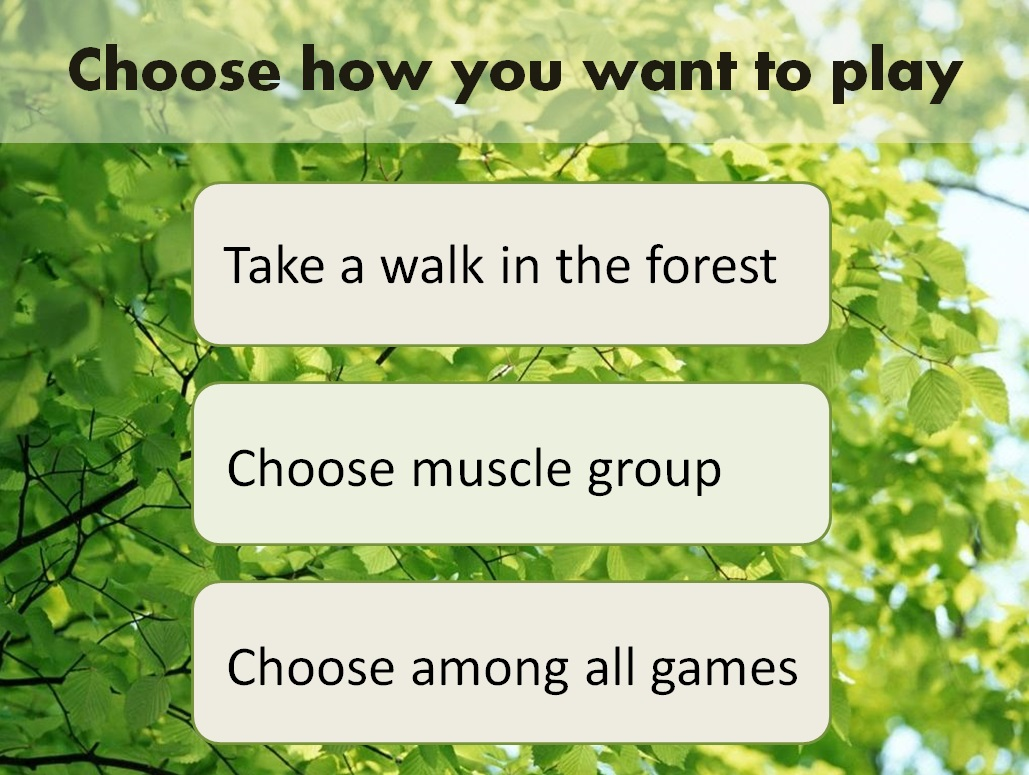
\includegraphics[scale=0.45]{choosePlay.jpg}
\caption[The menu - start]{In the first menu step, the player is given the opportunity to choose how they would like to play. The could go for the compounded game, playing according to a chosen muscle group, or they could choose among the four single games.}
\label{fig:menuStart}
\end{figure} 

\subsection{Exercises}
The activities we have selected for our exergame are based upon findings from workshop 1, and our own ideas, but the main reason for choosing these activities is because they involve exercises that are shown to be good for elderly. We have used \emph{Øvelsesbanken} \cite{eldretrening} as a guide to find exercises to use in our exergame concept. \emph{Øvelsesbanken} is created by the physiotherapy service in Trondheim, and consist of a set of exercises for elderly that increase balance and strength. This service is meant to be a tool to help physiotherapists set up customized programs for their older patients. We have picked out 18 exercises from \emph{Øvelsesbanken} that we feel will be a good foundation for our exergame concept. Some of the exercises chosen from \emph{Øvelsesbanken} are "picking apples" (or plums), "walking", and "rowing", see Figure \ref{walking}, \ref{rowing}, and \ref{pickingapples}. The remaining chosen exercises can be found in Appendix B. 

\begin{figure} [H]
\centering
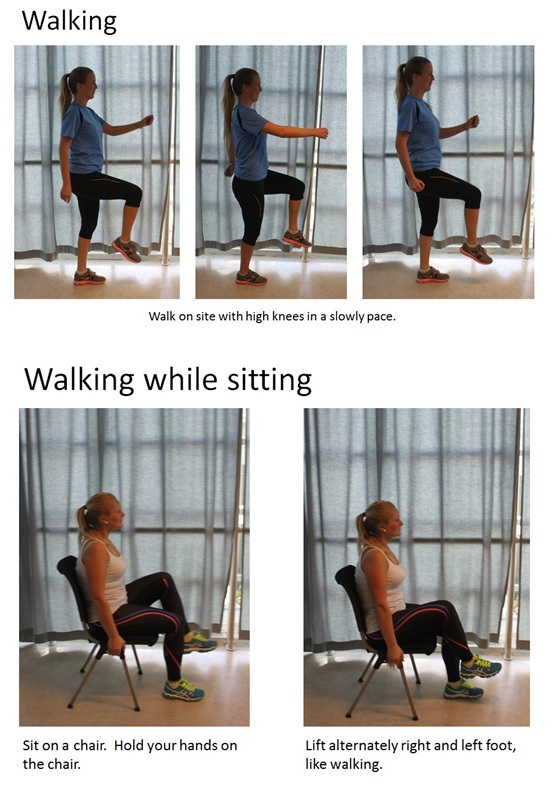
\includegraphics[scale=0.7]{Walking.jpg}
\caption[Exercise - walking]{}
\label{walking}
\end{figure} 

\begin{figure} [H]
\centering
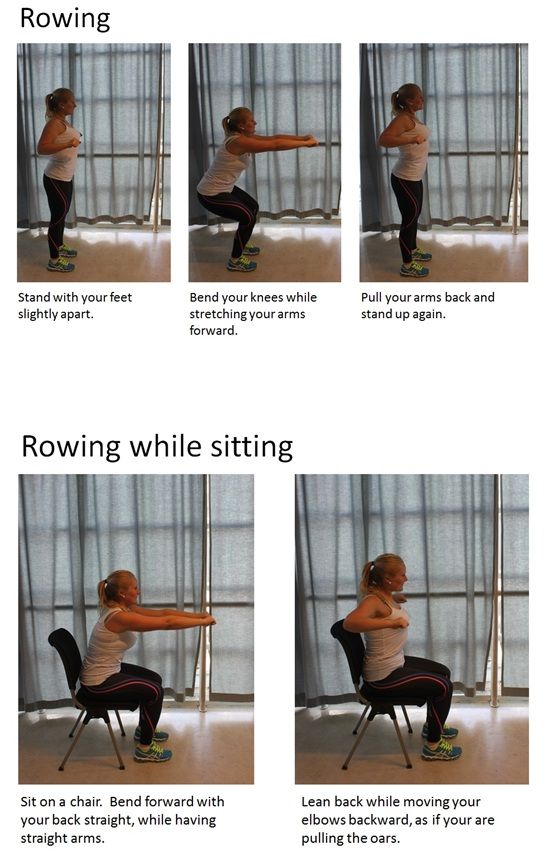
\includegraphics[scale=0.7]{Rowing.jpg}
\caption[Exercise - rowing]{}
\label{rowing}
\end{figure}

\begin{figure} [H]
\centering
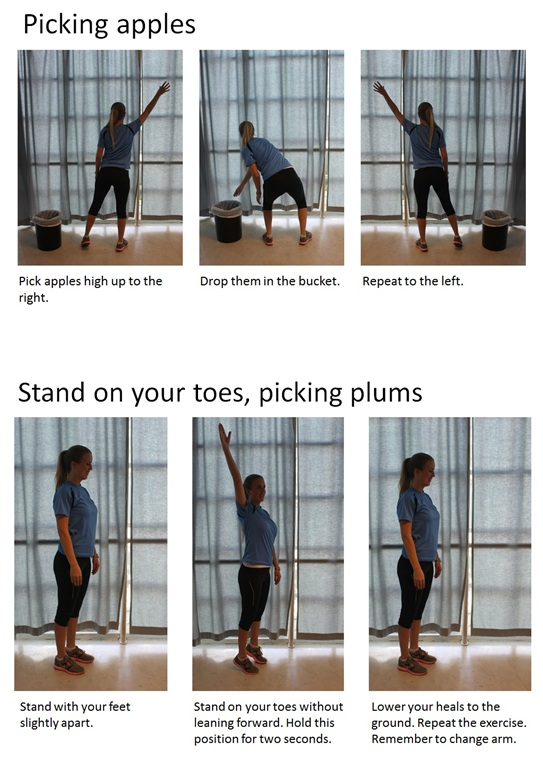
\includegraphics[scale=0.7]{PickingApples.jpg}
\caption[Exercise - picking apples and plums]{}
\label{pickingapples}
\end{figure}

\subsection{Information and instruction}
In this exergame concept the player will be given sufficient instruction and information about the technology, how to play, and how to perform the activities and exercises. When first starting the exergame the player will be given information on how to interact with the Kinect sensor and the game. The player will be told that they will have to use their body to engage game play, and that they will use their hand to navigate through the menu. Information will be provided on how to interact with the menu, like how to make a choice by "pressing a button". In the beginning of each of the five games there will be an instruction informing about the goal of the game, and how the player should move to perform the activities in the game. The information will not be given all at once, as this will require a lot of memorisation. Therefore, information will be given during game play, when situations occur that makes it appropriate to provide the player with new information. Every instruction will come with a button the player has to push to continue playing. In this way the players is in the control of the game, and they can decide for themselves when they are finished reading the information. Figure \ref{fig:kineintro} shows an example of an instruction. Players will always be given the possibility to skip the instructions, so that experienced players do not have to watch the same instructions every time they play.

\begin{figure} [H]
\centering
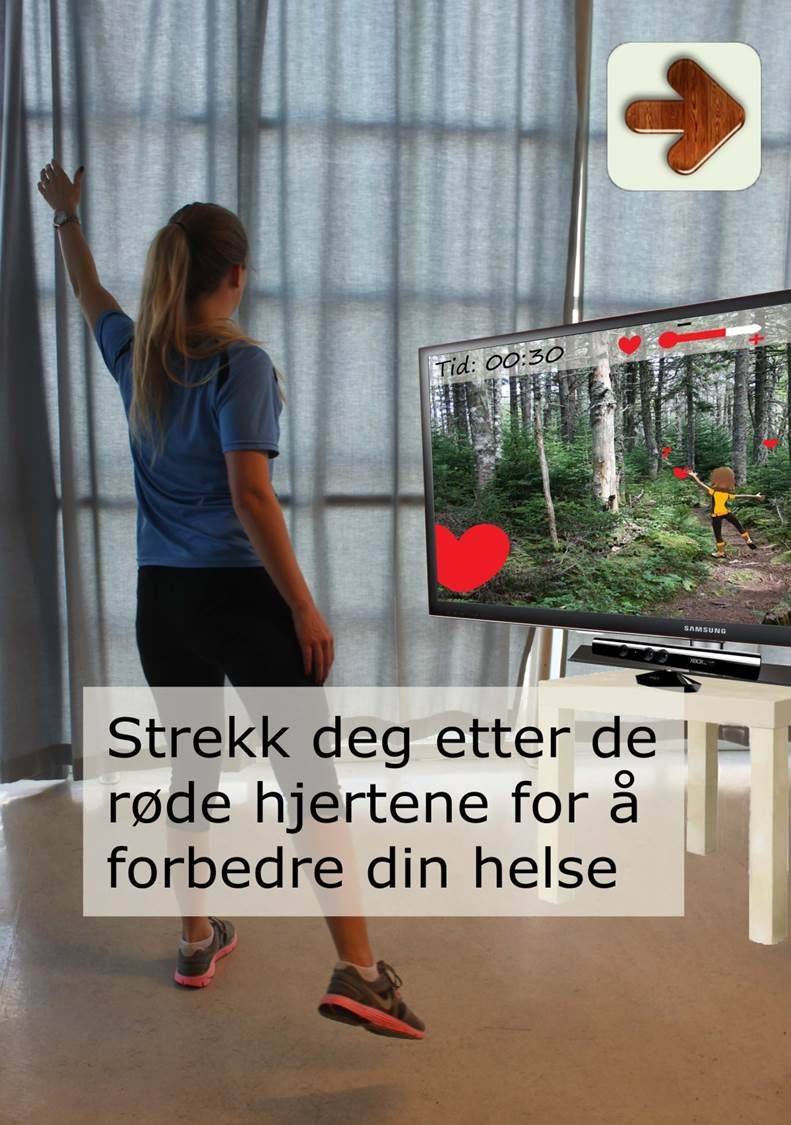
\includegraphics[scale=0.7]{KineIntro.jpg}
\caption[Instruction]{This figure shows an instruction in our exergame concept. The information given tells the player how and why to interact with the elements in the game, "reach for the red hearts to improve your health". There is a button up in the right corner. This will be used to continue on with the game when the player is done reading the information.}
\label{fig:kineintro}
\end{figure}

\subsection{Nature trail}
The main activity in "Out in the Nature", is what we have called a "Nature Trail". This involves a walk in the forest with quizzes along the way. The goal for the game is to complete the nature trail as fast as possible, while answering questions, and avoiding obstacles. Points will be given according to correct answers on the quiz, which will be shown up in the right corner together with a quiz icon. Because the Kinect sensor can track movement, points will also be given according to how well the player performs required movements. These points will not be shown as numbers, as movements will be difficult to measure and "grade". Therefore, gain from correct and well-performed movements are shown in a "health bar" on top of the screen. A red heart is shown together with the bar to represent health. Points for correct answers on the quiz are separated from points achieved from movements. This is because the quiz has to do with cognitive skills, while the latter is about physical skills. The time used to complete the nature trail will affect the final result of the "health bar", as this also reflects how well the player has moved during game play.   

Progress in the game requires movement, like walking as shown in Figure \ref{walking}. When walking, the avatar portraying the player will walk into the forest. The bigger movements the player uses, e.g. the higher the player lift their feet while walking, the higher pace, and more points s/he will achieve. Figure \ref{fig:hearts} shows a scene from the nature trail. Here we see an avatar in the forest, surrounded by hearts, where the avatar does a wide stretch trying to reach a heart. The hearts will be positioned so that it will require movement from the player to reach for them. Therefore, if the player gathers these hearts, his/her health will improve due to physical activity. Gain from gathering hearts will be shown in the "health bar".   

\begin{figure} [H]
\centering
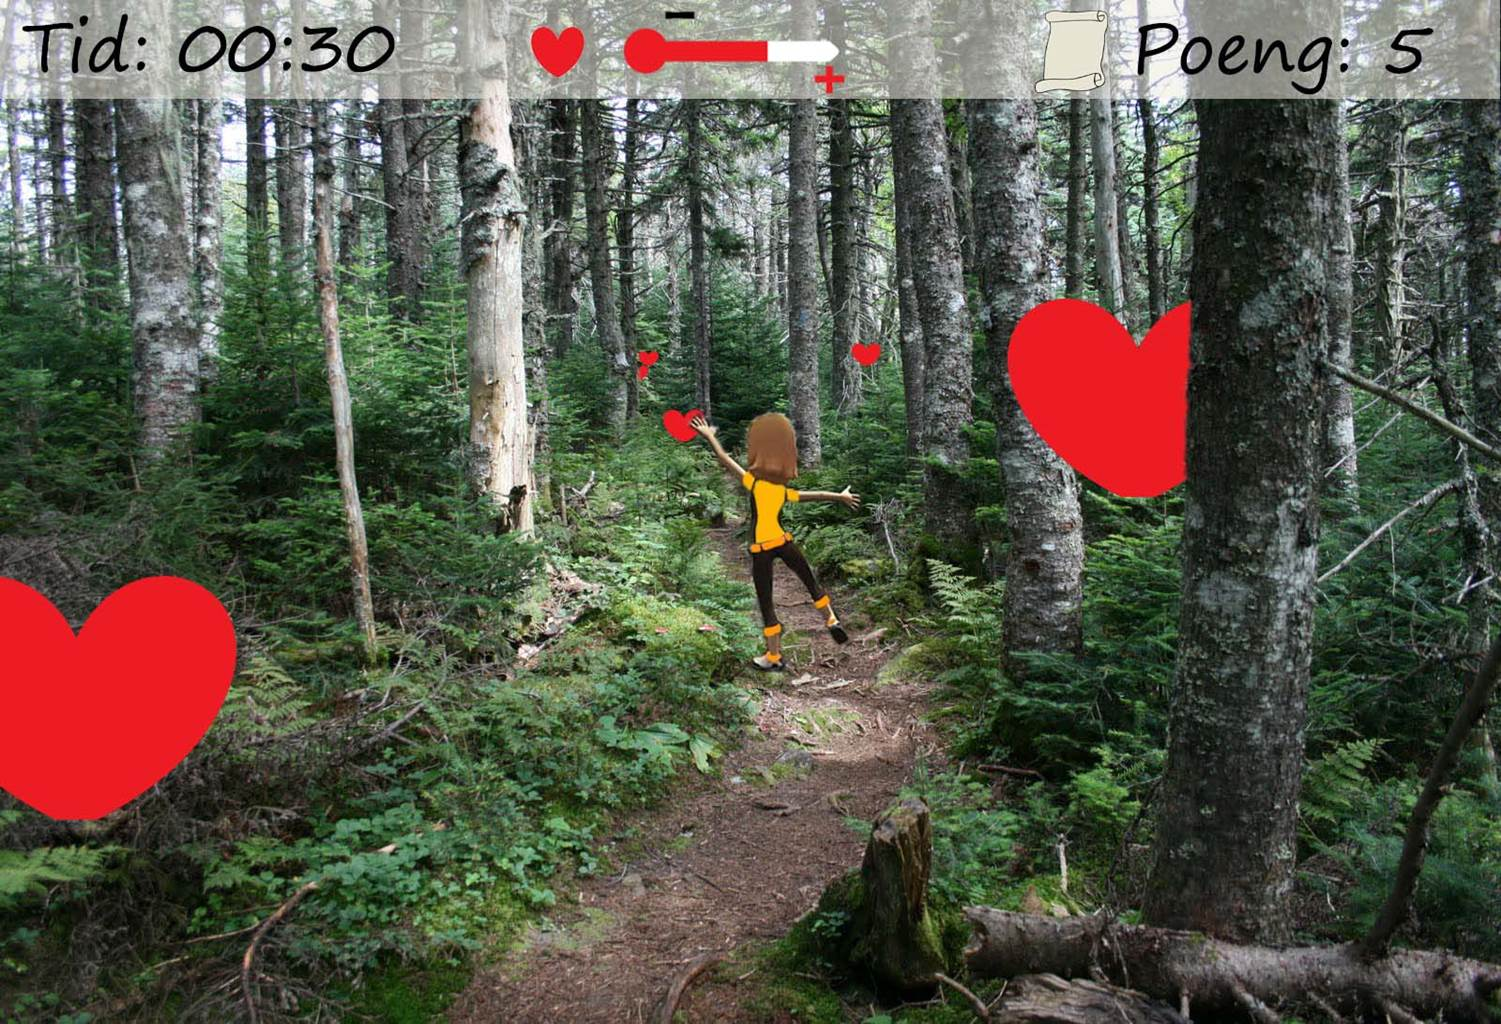
\includegraphics[scale=0.5]{hjerter.jpg}
\caption[Nature trail - stretching]{This figure presents a scene from the nature trail. We see an avatar in the forest, doing a wide stretch trying to reach a heart. This will result in improved health, shown in the "health bar".}
\label{fig:hearts}
\end{figure}

The quiz in this nature trail will be shown as pieces of paper hanging on trees, and the player has to reach for them to play, see Figure \ref{fig:quiz}. When picking a question, it will pop up and fill the screen. Possible answer alternatives will be shown, and the player will have to user their arm to navigate to what they believe is the right answer. The player does not have to answer the quiz to complete the nature trail, but it will affect the total score at the end. 

\begin{figure} [H]
\centering
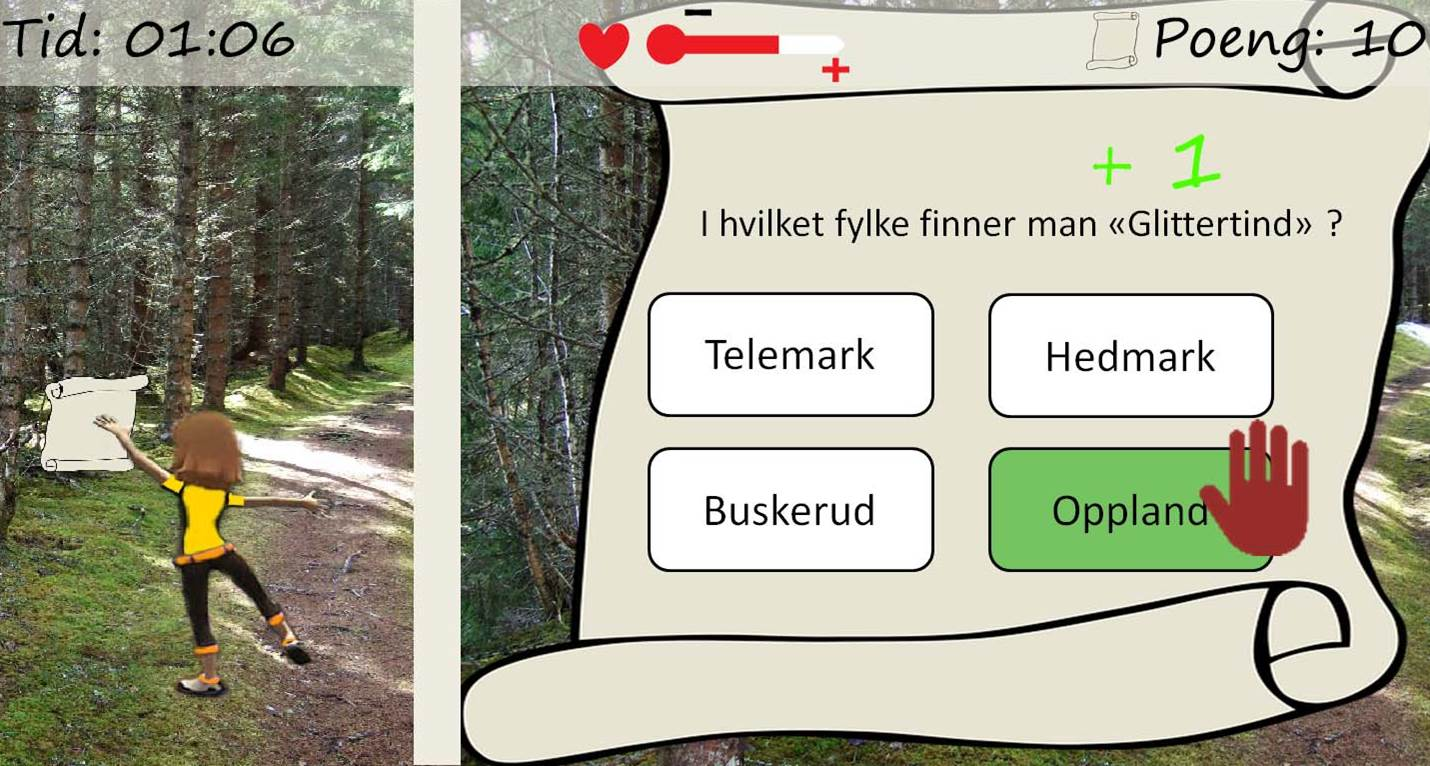
\includegraphics[scale=0.5]{quiz.jpg}
\caption[Nature trail - quiz]{The quiz in the nature trail will be shown as a piece of paper hanging on trees. Questions will pop up and fill the screen. Here, the player is asked about where to find the Norwegian mountain "Glittertind".}
\label{fig:quiz}
\end{figure} 

Along the way in the nature trail there will be various, natural obstacles that will force the player to move their body in certain ways to avoid them. The obstacles has been chosen according to which movements that are required by the player, as the nature trail is supposed to train the whole body. Examples of these obstacles is a river or creek that the player has to cross, or logs or rocks lying in the path that the player has to step over. To cross a river or creek the player has to balance on logs or step on rocks. This requires movements as toe-to-heel stepping, and step touch or skaters. When meeting a log, the player is required to take a big step, or a lunge, to get past it. Rocks in the path is avoided by performing sideways steps, or step touch. There will also be obstacles in head hight, like branches, which requires the player to go into deep squats to avoid them. After walking the nature trail for å while, the player will meet a lake. There will be a pier on the water, and by this pier there will be a rowing boat. To cross the lake, and continue the nature trail, the player has to take a side step and step into the boat. To move forward, rowing movements as shown in Figure \ref{rowing} are needed. There will be water lilies in the water which the player has to avoid. This is done by leaning the upper body over to the sides. All the described obstacles are shown in Figure \ref{fig:hindring1} and \ref{fig:hindring2}. The Kinect sensor will track the player's body, and increase or decrease the "health bar" according to how well the player perform the required movements. If the player would hit some of the obstacles, they will get a flash of red, indication that the player failed to avoid them. This is shown in the last picture in Figure \ref{fig:hindring2}. As a result, the "health bar" will decrease.     

\begin{figure} [H]
\centering
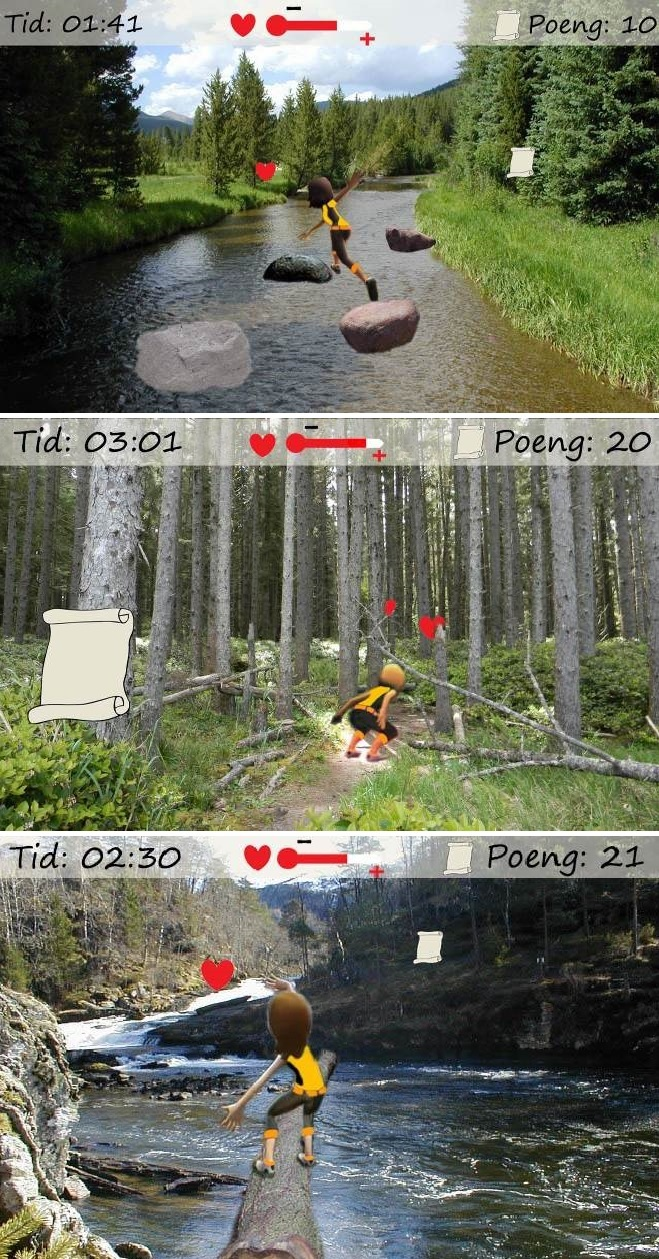
\includegraphics[scale=0.45]{hindring1.jpg}
\caption[Nature trail - obstacles, part one]{This figure present various obstacles to be found in the nature trail. We see the use of step touch or skaters to cross a creek, squats to avoid a branch, and toe-to-heel stepping to cross a river.}
\label{fig:hindring1}
\end{figure}

\begin{figure} [H]
\centering
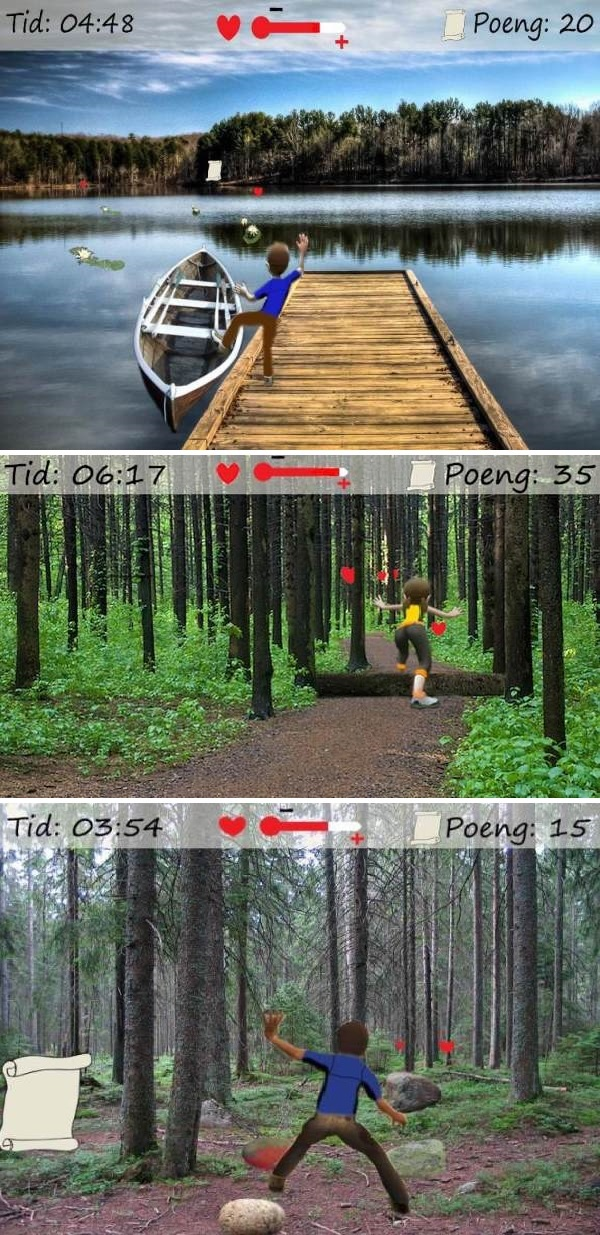
\includegraphics[scale=0.45]{hindring2.jpg}
\caption[Nature trail - obstacles, part two]{This figure present various obstacles to be found in the nature trail. We see an avatar taking a side step into a boat, the use of lunges to step over a log, and step touch to avoid rocks in the path.}
\label{fig:hindring2}
\end{figure}

Required movement during the nature trail we now have presented will exercise the whole body. This involves endurance, balance, and exercise of several muscle groups. This nature trail, with the quiz and movements combined, will be good for both cognitive skills and improved physical health.  

One of the requirements for this exergame concept is that the game has to show progress. In workshop 1, the informants told us that it was important to see that they learned something, and that they got better. It also was important to get the possibility to choose difficult levels themselves. We have solved this by having a step in the menu where the player can choose the preferred difficulty for the game, see Figure \ref{fig:omgivelseNivaa}. The nature trail offers three different forest environments to walk in, a pine wood, and two deciduous woods, showing both summer and fall. Within each environment, there are three difficulty levels, easy, medium, and hard. First time playing, only the easy level will be available. The higher levels will be unlocked when the player is "good enough".   

\begin{figure} [H]
\centering
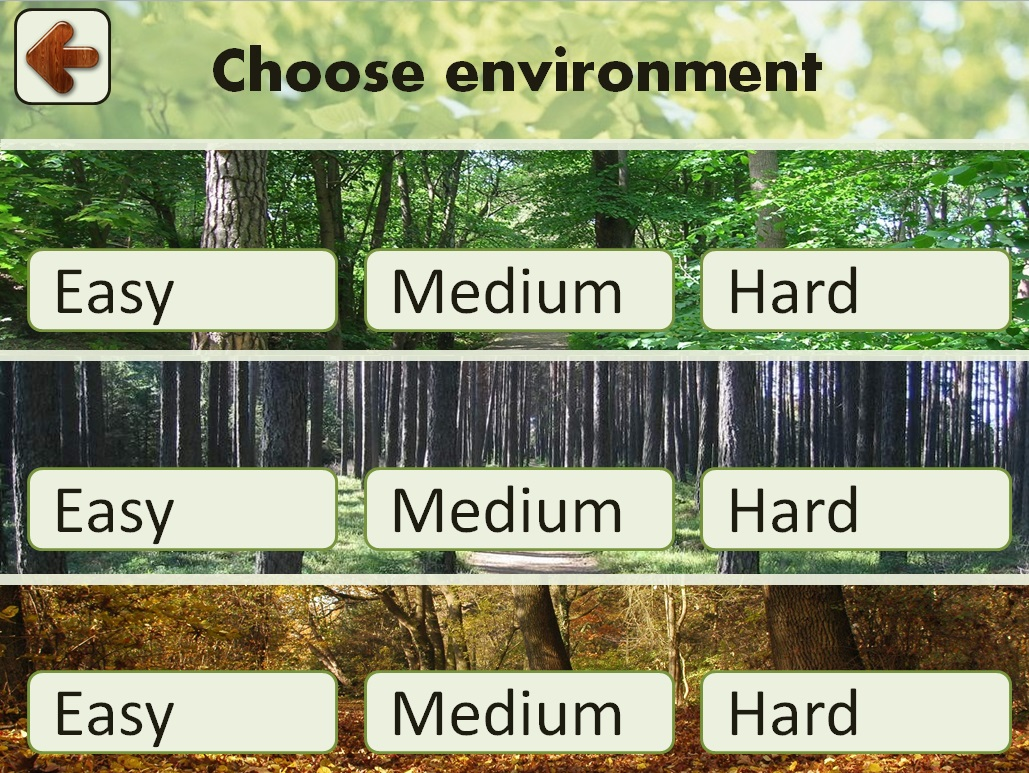
\includegraphics[scale=0.45]{chooseEnvironment.jpg}
\caption[Choice of environment and difficulty level]{When "Take a walk in the forest" is chosen, players will get the possibility to choose environment and difficulty level. The environments to choose from are pine wood, deciduous wood summer, and deciduous wood fall. Within each environment there are three difficulty levels, easy, medium, and hard.}
\label{fig:omgivelseNivaa}
\end{figure}
     

\subsection{The Four Single Games}
In addition to the nature trail, "Out in the Nature" consists of four shorter games with focus on completing one single activity or challenge. The activities we have chosen for our exergame concept is wood chopping, paddling down a river, swimming in a lake, and picking apples. Within every game the player has the possibility to choose number of players and difficulty level. In multi player mode, players can choose if they want to cooperate or compete against each other. When competing, the players will have the possibility to select difficulty level individually. This is to allow for players with different experience to play together, like an elderly and his/her grandchild. Figure \ref{fig:velgSpill} shows how these single games will be presented in a menu. We will describe one of these four games in more detail.

\subsubsection{Picking Apples}
"Picking Apples" is a game that requires squats and stretch exercises, which will strengthen balance and muscles in thighs and the gluteal area. The goal for this game is to pick as many red, ripe apples as possible in a given amount of time. The apples should be put in baskets on the ground. Picking apples requires stretching, and to assure that the picked apple end up in the bucket, the player has to perform squats, see Figure \ref{fig:appleStretch} and \ref{fig:appleSquat}. When apples first appears on the tree they will be green, indicating that they are not ready to be picked. If ripe apples are left hanging on the tree for too long, they will rot and fall to the ground. Rotten apples will have a brown color. Figure blabla shows a prototype of what this game will look like.  

\begin{figure} [H]
\centering
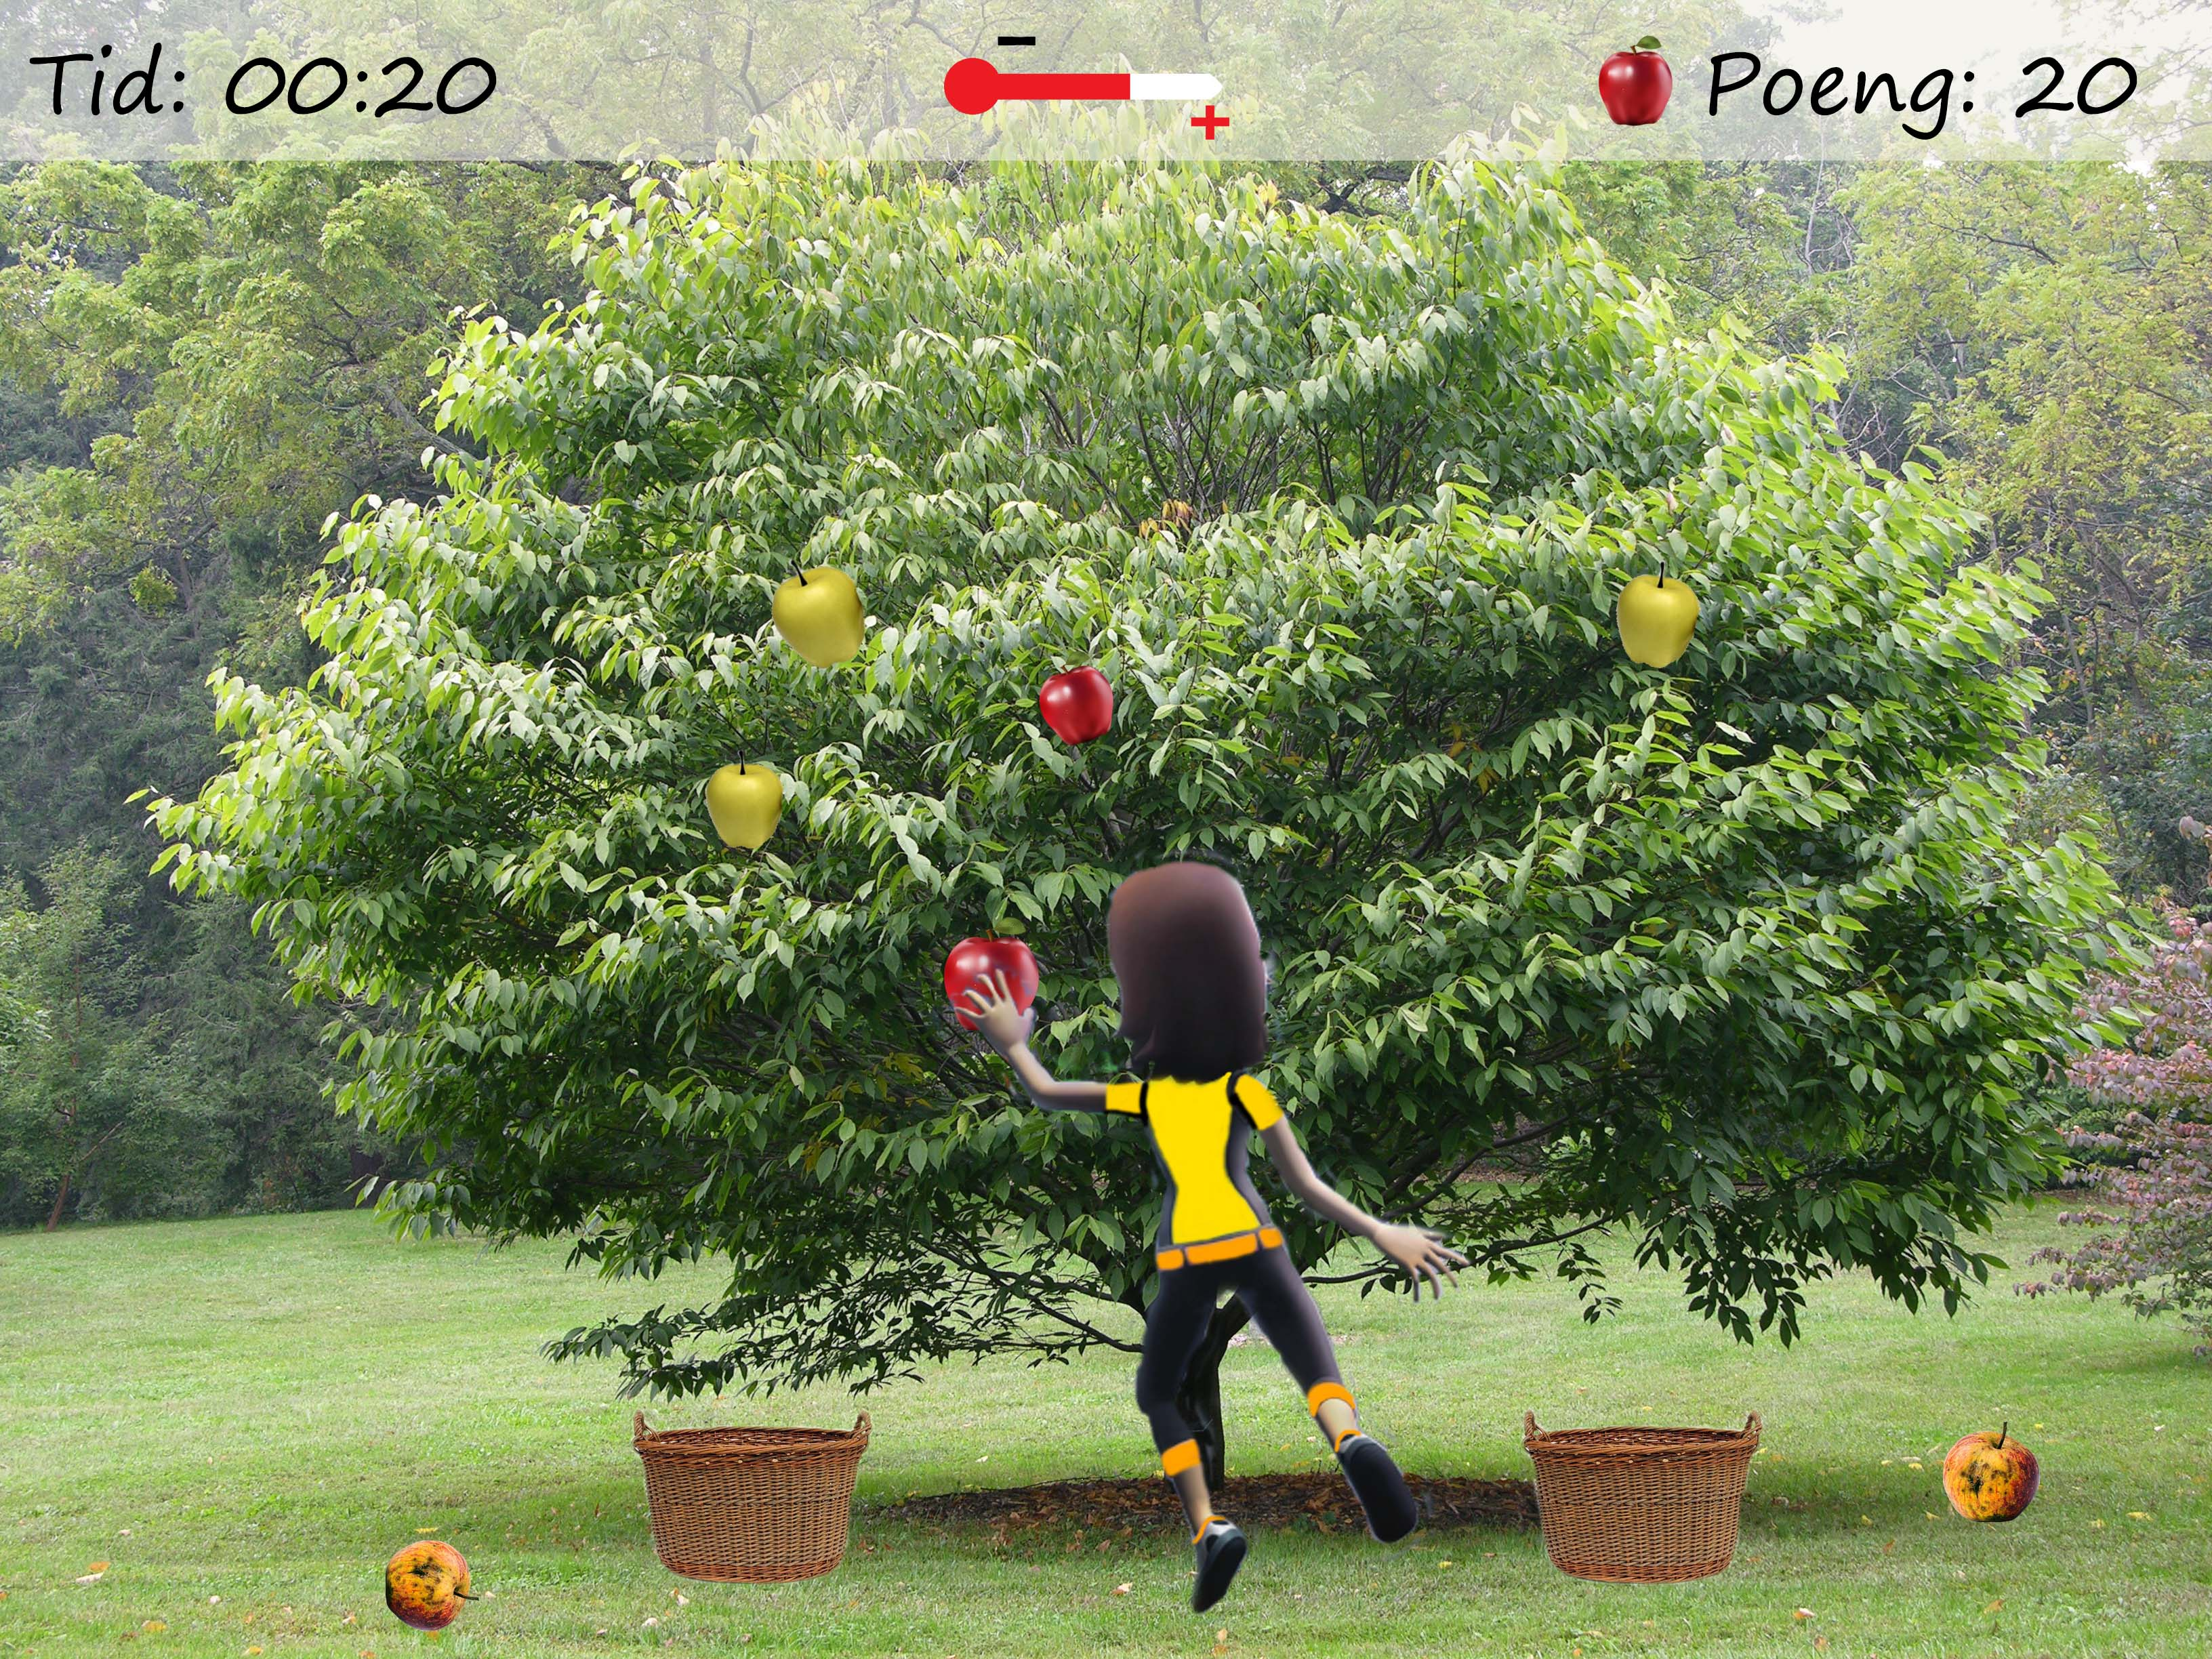
\includegraphics[scale=0.1]{gameappletree.jpg}
\caption[Picking apples - stretching]{The player stretch up to pick a red, ripe apple. We observe that there are, in addition to red apples, three green apples on the tree, and two rotten on the ground.}
\label{fig:appleStretch}
\end{figure}

\begin{figure} [H]
\centering
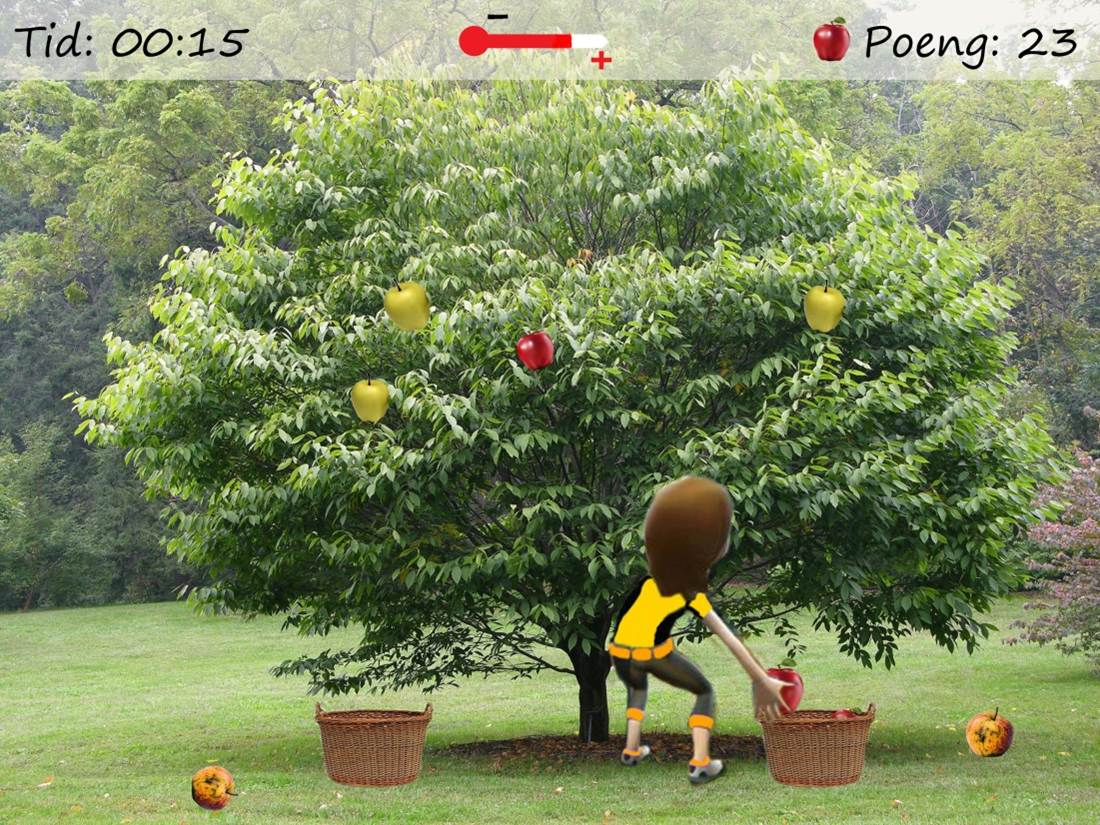
\includegraphics[scale=0.45]{squateple.jpg}
\caption[Picking apples - squats]{The player has picked a red apple and is about to put it in the bucket. The player use deep squats.}
\label{fig:appleSquat}
\end{figure}

Points will be given according to how many apples the player has picked, see Figure \ref{fig:appleOver}. 3 points will be given for each ripe apple that is picked and put in a basket. The player will loose points if green apples are picked, or if apples have been given the time to rot. Green apple picked will result in -1 point, and rotten apples will give -2 points. If the player does not perform squats when putting apples in a bucket, there is a great possibility that the apple will miss the bucket and fall to the ground. This will give the same loss of points as a rotten apple, -2 points.       

\begin{figure} [H]
\centering
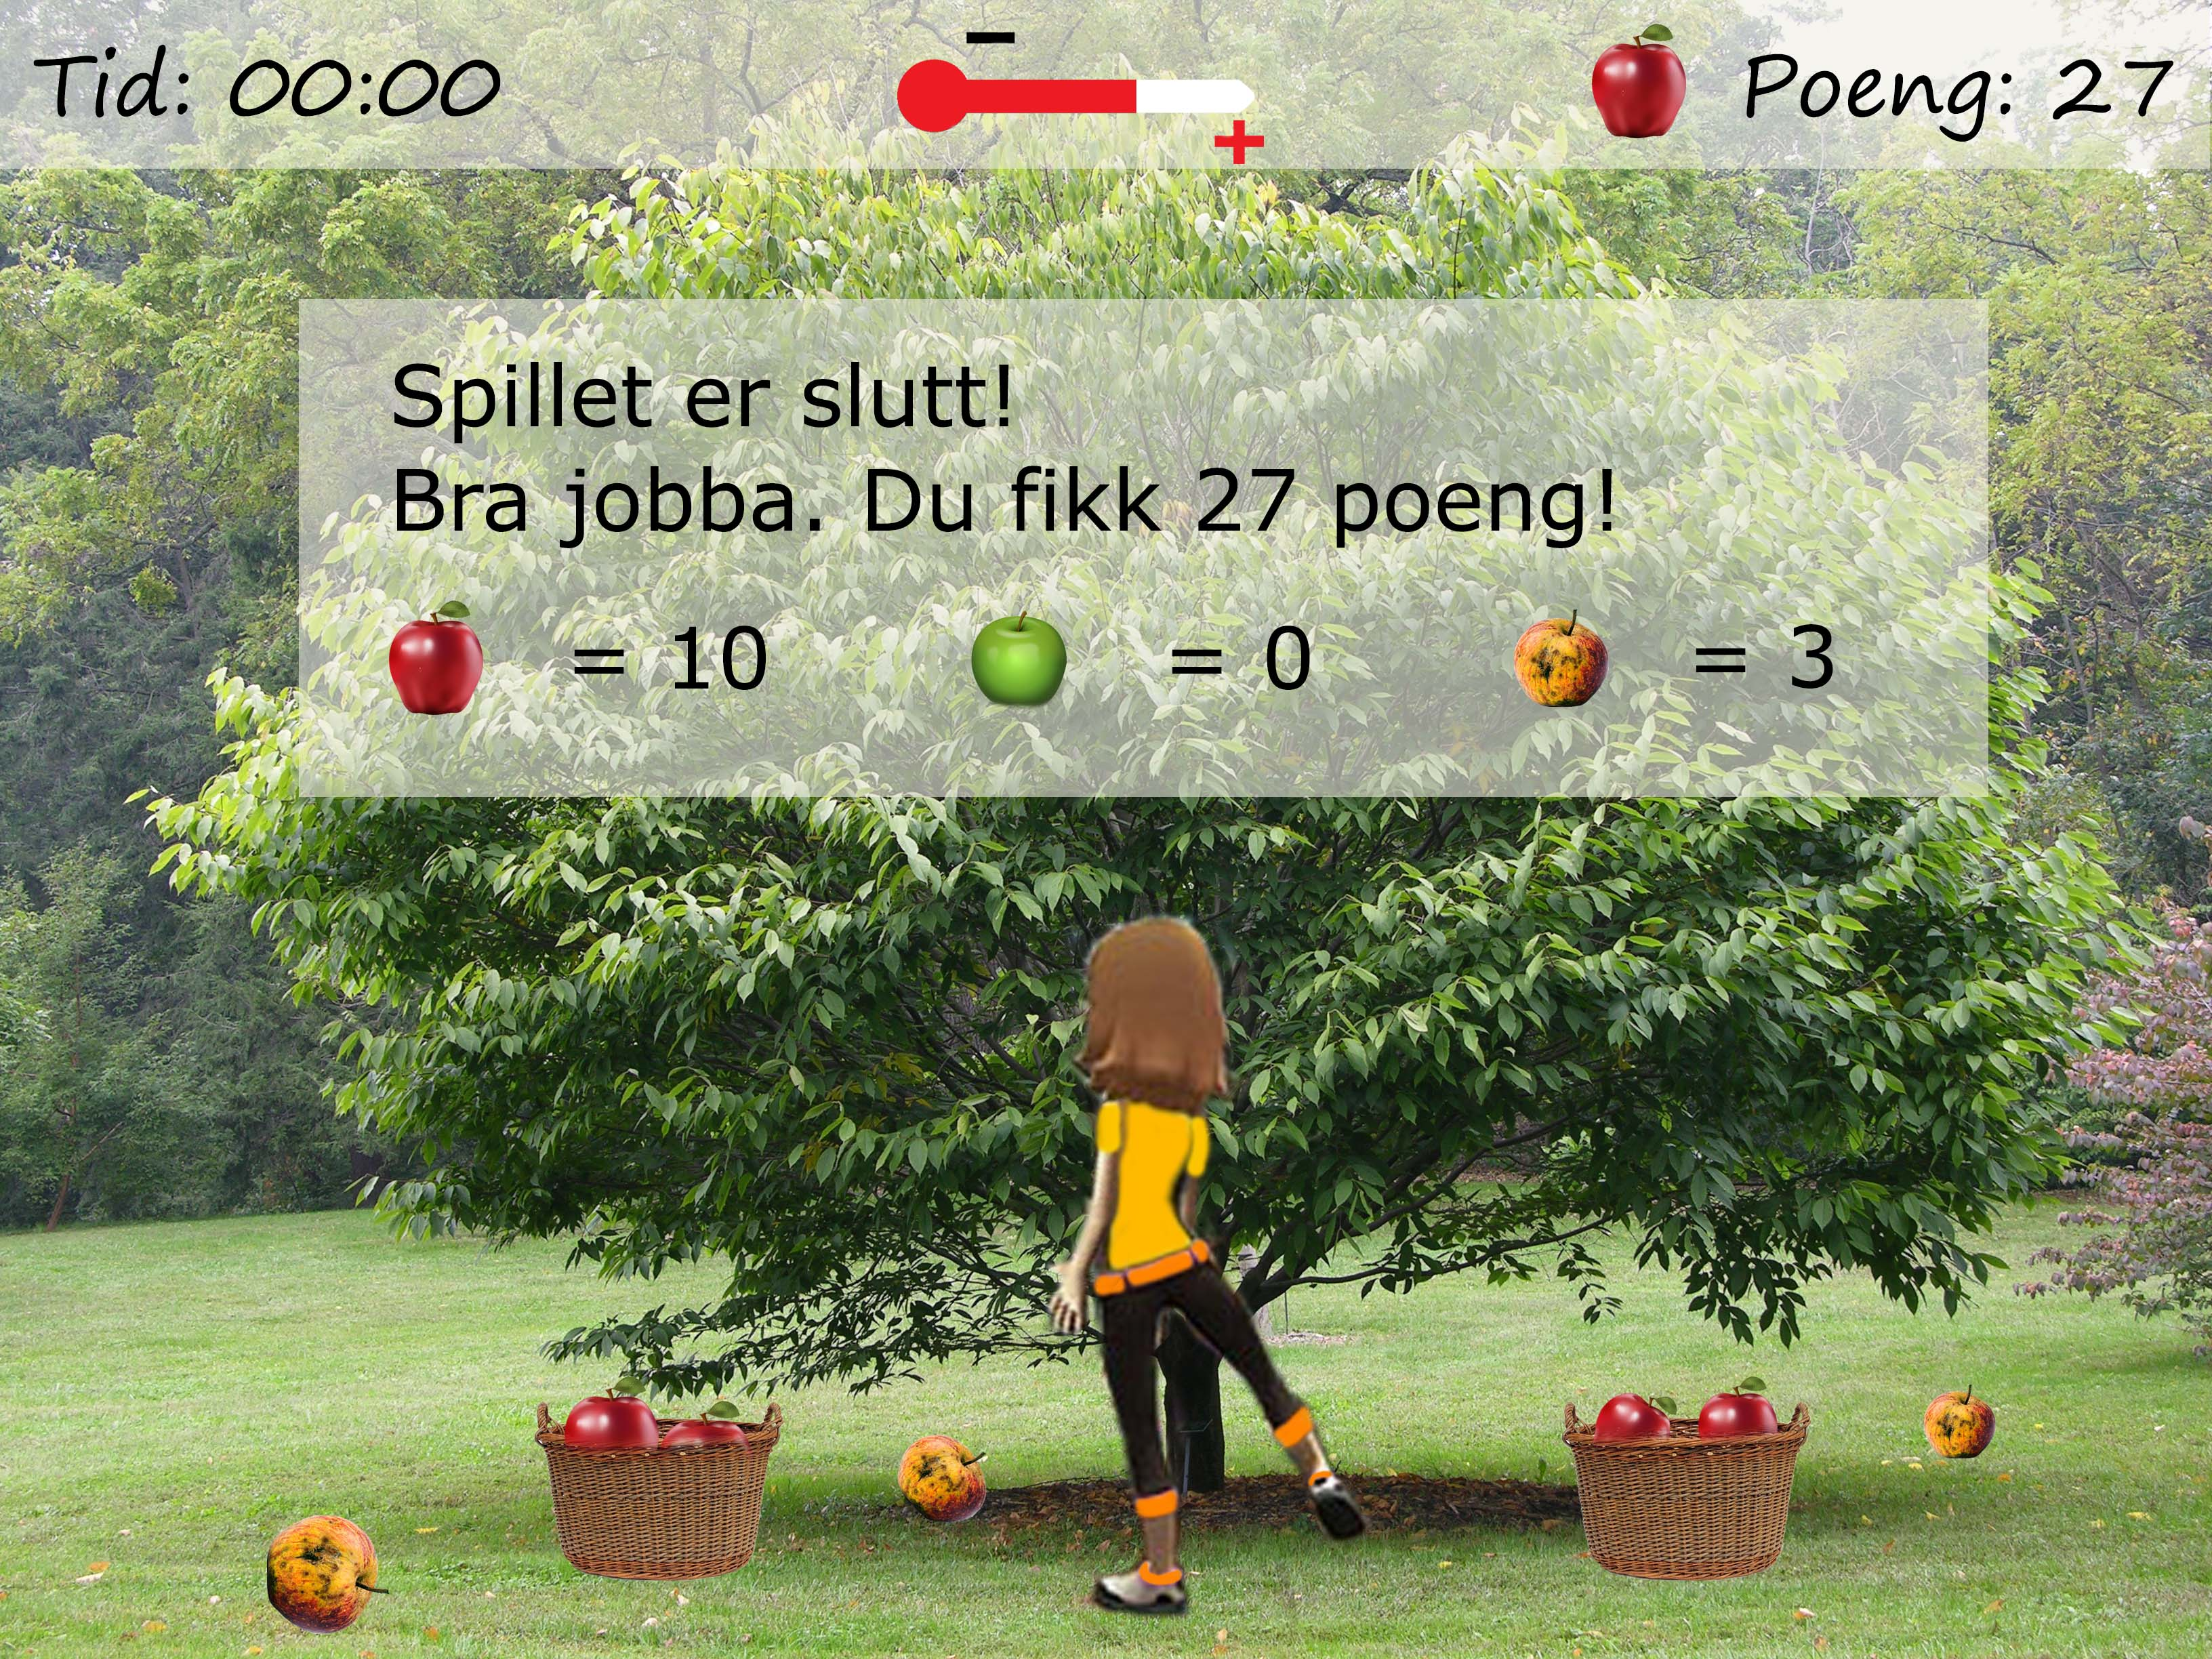
\includegraphics[scale=0.1]{appletreeend.jpg}
\caption[Picking apples - points]{This figure represent a final scene in the "picking apples" game. The text "The game is over! Good work. You achieved 27 points!", in addition to number of apples picked, are shown.}
\label{fig:appleOver}
\end{figure}

Apples will appear on the tree and grow in a certain tempo according to the chosen difficult level. Higher difficulty will result in more apples on the tree at the same time, and a faster ripening rate. An extra challenge to be added at a higher difficulty level is requirements to which of the two buckets the newly picked apple should be put. This is to train cognitive skills and to include more variation in movements and exercises. This game allows for multi player mode where the players could collaborate on picking apples, or compete on who that can pick the most apples, see Figure \ref{fig:appleMultiplayer}. 

\begin{figure} [H]
\centering
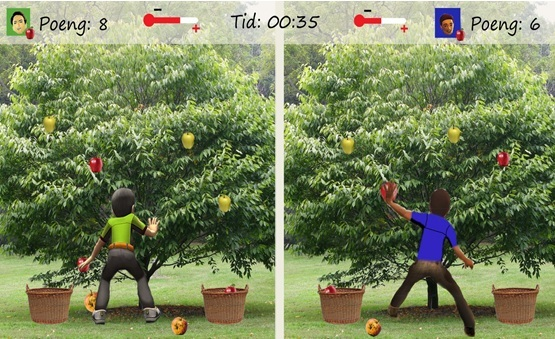
\includegraphics[scale=0.8]{multiplayereple.jpg}
\caption[Picking apples - multi player]{In this figure we observe two players playing together in competitive mode.}
\label{fig:appleMultiplayer}
\end{figure}

\subsection{The Menu}
\label{sec:menu}

One of the main problems we observed during workshop 1 was related to handling the menus in the various games they played. The general perception from workshop 1, in addition to our own experience from playing, was that the menus were complex, difficult to follow, demanding to navigate through, and that they were too sensitive. Therefore, we have made a prototype for a menu, which we will present in this section. The menu prototype is developed with Microsoft PowerPoint.

The design of our menu proposal is based upon the interface requirements, findings from workshop 1, and theory about designing interfaces for elderly. Simple design, distinct elements, and easy to read information are emphasised to make it user-friendly for elderly that might suffer from declined vision. It has been a focus not to have too much information in each menu step. We have therefore chosen to make a menu consisting of more steps, rather than filling few menu steps with lots of information and choices.   

The menu starts with the choice of how you want to play. The player could choose between a walk in the forest, to exercise a preferred muscle group, or the player could choose between the four single games. If the player wants to play according to training a specific muscle group, s/he will be given the choice of which muscle group to exercise. Independent of how the player choose how to play, s/he will be given the opportunity to choose difficulty level and number of players for the game. Figure \ref{menu1} and \ref{menu2} goes through the menu, from start, through choosing muscle group, to ending up playing "Picking Apples". As seen from what we have presented this far, the menu includes a lot of choices. This is based on the informants feedback in workshop 1, where they said that they would have the possibility to make their own choices. They did not want the game to control them.   

\begin{figure} [H]
\centering
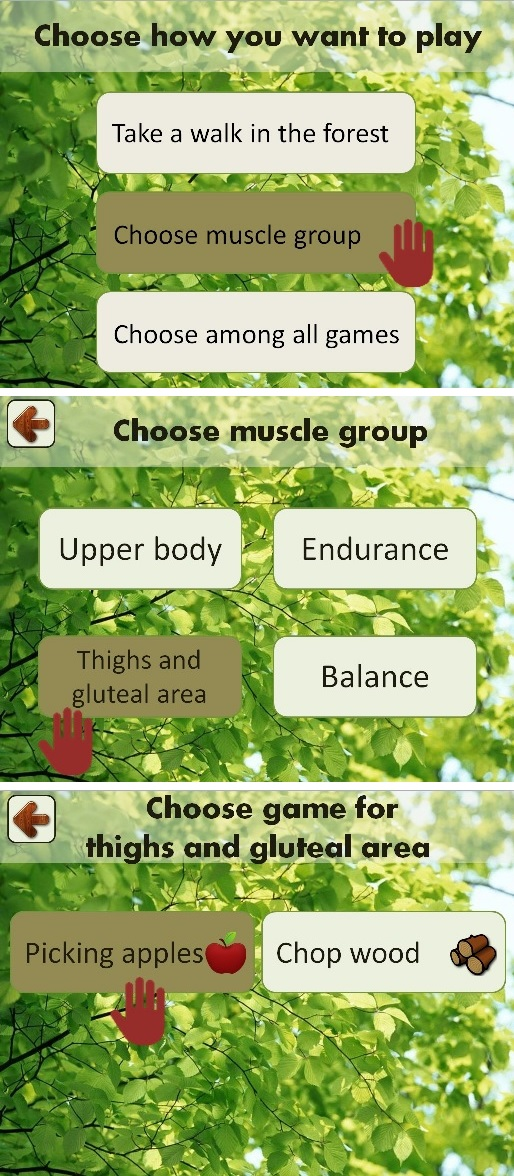
\includegraphics[scale=0.45]{menuEnglishStep1.jpg}
\caption[Menu review -  part one]{This figure shows the menu step by step, from the beginning to playing a single game, here picking apples. The selection of single games is a result of the chosen muscle group.}
\label{menu1}
\end{figure}

\begin{figure} [H]
\centering
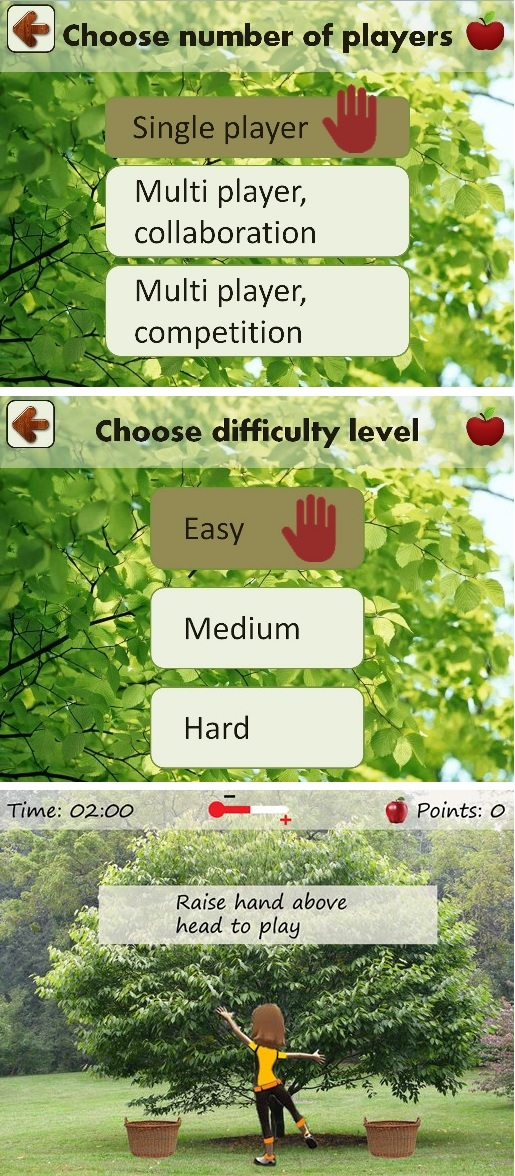
\includegraphics[scale=0.45]{menuEnglishStep2.jpg}
\caption[Menu review - part two]{This figure shows the menu step by step, from the beginning to playing a single game, here picking apples. Single player game and difficulty level easy are chosen. When ready to start the text "raise hand above head to play" is shown.}
\label{menu2}
\end{figure}

Figure \ref{fig:velgSpill} shows a step from the menu and the different menu elements. We have used a range of green colors, and a picture of green leaves as background, to create a theme related to forest and nature. Menu buttons are arranged as list elements or in a square, depending on what is most appropriate. The size of the elements are chosen with usability in mind, there should be room for a proper font size, and it should be easy to push the right button. The buttons have a light green, almost white, background color, with a darker green outline. The text is written in black with an easy-to-read, sans serif font. The contrast between button background and text color is chosen with respect to design guidelines for elderly, presented in Section \ref{sec:designelderly}. The chosen colors is also based on \cite{blindeforbundetTekst}. Taking the element's surroundings into account when choosing colors is important if you will make the element stand out. With e.g. green vegetation as surroundings, white background color, with black, dark green, or dark blue text should be chosen to create maximum contrast.   

\begin{figure} [H]
\centering
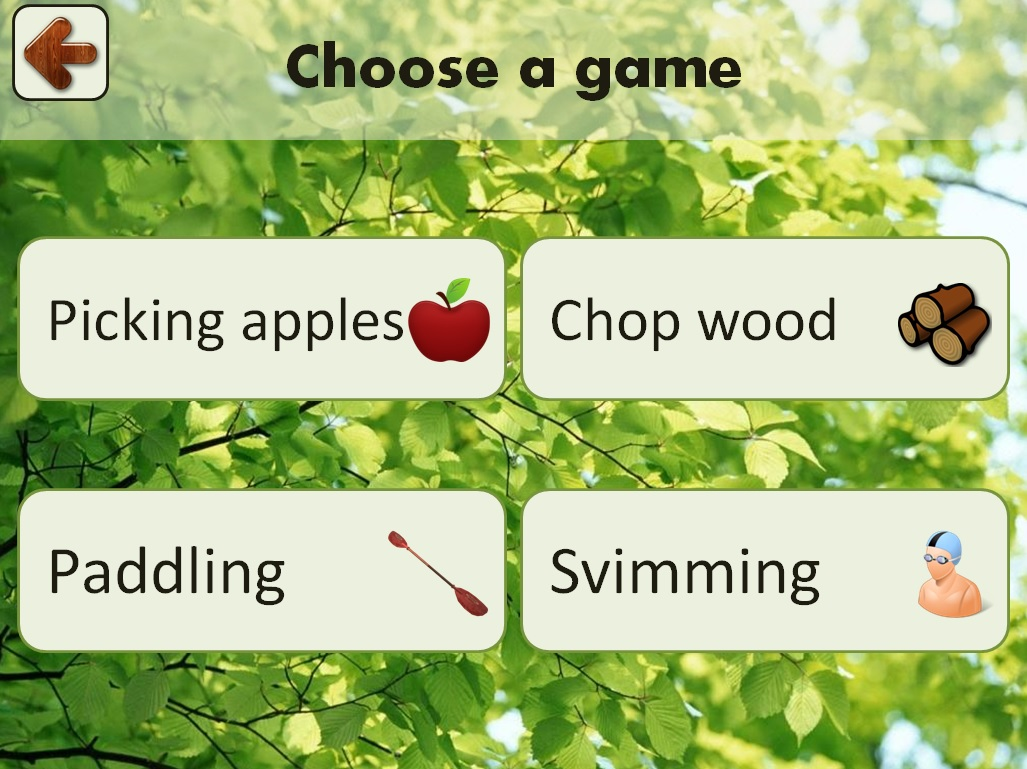
\includegraphics[scale=0.4]{chooseGame.jpg}
\caption[The four single games]{Besides the walk in the nature the players can choose between four single games, picking apples, chopping wood, paddling, and swimming.}
\label{fig:velgSpill}
\end{figure}

The title on each step is written in a bold, black, easy to read font, on a semi-transparent light-colored background. The title is stating what choice to be made at the current step. From the Eight Golden Rules presented in Section \ref{sec:designguide} we know that it is important to have an interface with visible information. These rules also states that users always should be given feedback on their actions. In addition to this, there was a general opinion at workshop 1 that the informants wanted to see clearer response on their actions. We have included this in our concept by highlighting elements that are "in action", see Figure \ref{fig:avatarAction}. The player's hand movements are portrayed on the screen as an avatar hand. The avatar hand has been given a clear color and a solid fill. This has been done to avoid having the same diffuse avatar hand as in the personal trainer game.  

\begin{figure} [H]
\centering
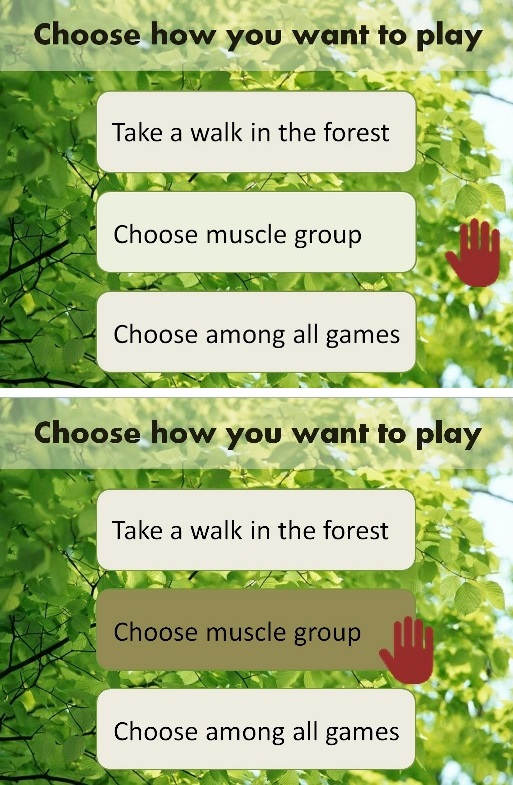
\includegraphics[scale=0.5]{menuAction.jpg}
\caption[Menu - Action and response]{In this figure an avatar hand is shown. The avatar hand will react according to the player's movements. We see that when the player move their arm over an element, it will change color.}
\label{fig:avatarAction}
\end{figure} 

Up in the left corner there is a back button, which will make it possible for users to always regret their action. The permission to reverse actions is also an important guideline from the Eight Golden Rules. The back button is shaped and colored as the other menu buttons to maintain consistency and intuitiveness. The choice of placement is based on guidelines stating that navigation should be on top, and on the natural way to read and observe information, which is from top to bottom, from left to right [KILDEee]. We avoided placing the back button in the bottom left corner to not mix it with the cancel/pause feature included in the Kinect software (holding your left hand straight 45 degrees from your body). The back button is marked with a wooden arrow, a familiar and intuitive icon related to navigation. The choice of using an wooden arrow is based on its relation to our forest theme. 

In the menu step where the player should choose between the four single games, we have used icons in addition to text on each button, see Figure \ref{fig:velgSpill}. The icons represents the challenges in each game, and they are meant to make it easier for the player to understand the game behind the button. When choosing a game, e.g. "picking apples", the icon will follow up in the right corner, to inform the player where s/he is headed, and to reduce memory load. This is shown in Figure \ref{fig:iconEple}.  

\begin{figure} [H]
\centering
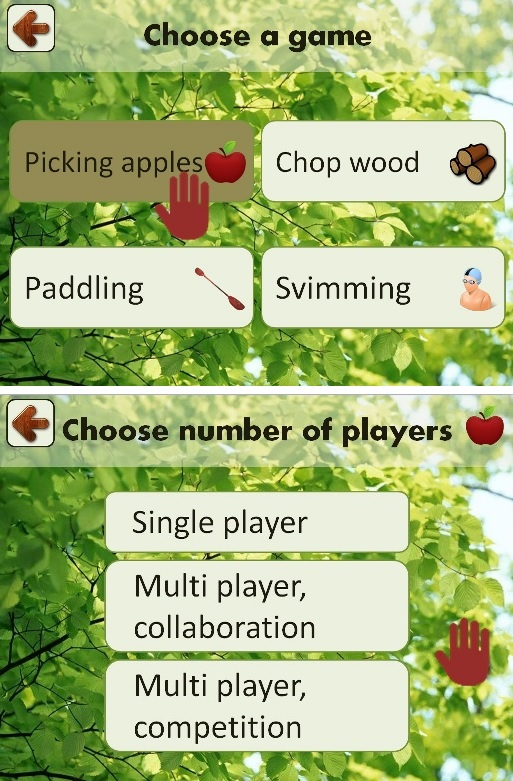
\includegraphics[scale=0.5]{menuIconApple.jpg}
\caption[Menu - use of icons]{In this figure we see that icons from menu buttons will follow the rest of the menu. Here we see that the apple icon will follow into the menu step where number of players are to be chosen.}
\label{fig:iconEple}
\end{figure} 
     
\subsection{A Video Game Series}
In our idea of a video game concept, our "out in the nature" exergame is a part of a video game series called "Kinect Experiences", see Figure \ref{fig:videogameseriesAlone}. This "Kinect Experiences" series consist of 4 individual games with the same structure as the game we have already presented. This means, one compounded game and four single games. The difference between the four video games are the main themes. In addition to "out in the nature", the "Kinect Experience" series consist of the video games "farm life", "on vacation" and "in the mountains". The five games within each video game will consist of activities that are connected to the main theme of each video game, like the exergame we already have presented. Examples of single games could be gathering eggs, and stacking hay bales in "farm life", and it could be a walk on the beach, or catching gold fish with a hoof in "on vacation". The idea behind this video game series is to offer a wide range of games, activities and exercises that fits the various interests the user group have. What this video game series would look like on Xbox's website is shown in Figure \ref{fig:videogameseriesHele}. The price presented is only an example. 

\begin{figure} [H]
\centering
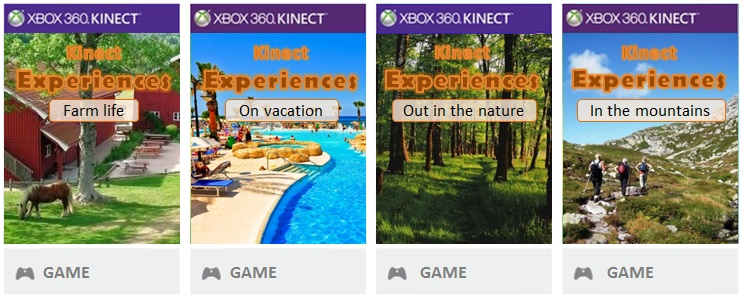
\includegraphics[scale=0.65]{videoGameSeriesAlone.jpg}
\caption[Presentation of our video game series]{A presentation of our video game series "Kinect Experiences" [modified from \cite{XboxNettside}].}
\label{fig:videogameseriesAlone}
\end{figure}

\begin{figure} [H]
\centering
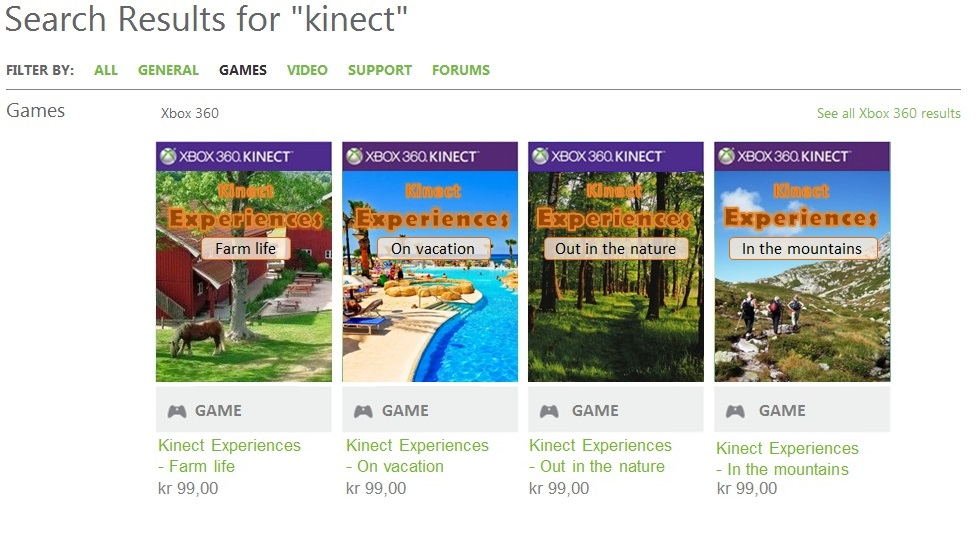
\includegraphics[scale=0.5, angle=90]{videoGameSeries.jpg}
\caption[Presentation of our video game series in a Xbox website view]{A presentation of how our video game series would look like on Xbox's website [modified from \cite{XboxNettside}].}
\label{fig:videogameseriesHele}
\end{figure}



\section{Miscellaneous Aspects to Consider About the Exergame Concept}
\label{sec:misc}

Delay
Fysioterapeuter
Enkelt å sette opp
Lastetid. Hente fram instruksjonsvideo først, og laste opp spillet mens denne vises?

\begin{table} [H]
\label{tab:nfunc2}
\centering
    \begin{tabular}{|l|l|}
 
       \hline
The system shall be able to run on both PC and Xbox. \\ \hline
The system shall be easy to set up (physically).\\ \hline
The system shall include Kinect functionality, like pausing \\ a game by holding one arm out from the body. \\ \hline
The system shall load within few seconds.\\ \hline
The system shall be small in size and do not require too \\ much space.\\ \hline
The system shall not require too much capacity. It shall \\ be able to run on a regular PC. \\ \hline
The system shall not require too much power. \\ \hline
The system shall avoid delay between the player's \\ movement and action on the screen.\\ \hline
The system shall ensure secure storage and sharing of \\ profiles. \\ \hline
    \end{tabular}
    \caption[Miscellaneous non-functional requirements]{Miscellaneous non-functional requirements}
\end{table} 
